\section{Extensions and improvements}
Two variants of the algorithm have been discussed earlier in the thesis, with different purpose and functionality.
Benchmark data was produced for these variants as well, but on a limited subset of the problems, chosen specifically to test the variants and their intended purpose.
Results for both variants will be reviewed in in order to determine if they have the desired effect, and if their function is satisfactory with respect to the drawbacks they introduce.
Results will be presented by comparison with the original benchmark only, without the solvers benchmarked by \textcite{deGivry14}.

% [review] - rest of this file may be osammanhängande

\subsection{The \enquote{push} operation}
The purpose of the \enquote{push} operation is to decrease the optimality gap of the approximative algorithm once a feasible solution has been found.
Six problem sets from \cref{tab:comparative-results} were therefore chosen for this benchmark, all with comparatively bad solutions (optimality gaps close to or above \SI{1}{\percent}) but competitive runtimes.
The expectation was to obtain better solutions while maintaining good runtimes.

\begin{table}[b!]
	\centering
	% Updated 2014-05-24
	\caption{
		Optimality gap and runtime using the \enquote{push} operation.
		For several chosen problem sets, the \enquote{push} variant runtime is compared to the results obtained by the standard algorithm (see \cref{tab:comparative-results}).
	}
	\label{tab:push-results}
	\begin{figcenter}
	\begin{tabular}{xySSS[round-mode=places,round-precision=3,scientific-notation=fixed,fixed-exponent=0]
				     S[round-mode=places,round-precision=3,scientific-notation=fixed,fixed-exponent=0]
				     S[round-mode=places,round-precision=2,scientific-notation=fixed,fixed-exponent=0]
				     S[round-mode=places,round-precision=2,scientific-notation=fixed,fixed-exponent=0]}
		\toprule
			{} & {} & \multicolumn{2}{c}{\(\#\) solved} & \multicolumn{2}{c}{Gap (\si{\percent})} & \multicolumn{2}{c}{Mean time (\si{\second})} \\
			\cmidrule(rl){3-4} \cmidrule(rl){5-6} \cmidrule(rl){7-8}
			{\normalsize Category} & {\normalsize Set} & {Std.} & {\enquote{Push}} & {Std.} & {\enquote{Push}} & {Std.} & {\enquote{Push}} \\
		\midrule
\acrshort{cfn}	&	Pedigree	&	10	&	10	&	1.804874e-00	&	1.51249400	&	2.3750	&	5.6070 \\
\acrshort{cvpr}	&	GeomSurf	&	600	&	600	&	2.091307e-00	&	2.09130700	&	0.0460	&	0.0425 \\
				&	SceneDecomp	&	715	&	715	&	7.545481e+01	&	75.4547890	&	0.0210	&	0.0170 \\
Max-\acrshort{csp}	&	BlackHole	&	37	&	37	&	9.009009e-01	&	1.08108100	&	58.8900	&	31.3310 \\
				&	Langford	&	4	&	4	&	1.311265e-00	&	1.55417600	&	70.7775	&	56.2925 \\
				&	QCP	&	60	&	60	&	1.292034e-00	&	1.30359500	&	43.2575	&	38.0705 \\
\acrshort{mrf}	&	ObjectDetection	&	37	&	37	&	6.465565e-00	&	6.46556500	&	279.8620	&	167.0170 \\
		\bottomrule
	\end{tabular}
	\end{figcenter}
\end{table}

\Cref{tab:push-results} shows the results of benchmarking the \enquote{push} operation on the selected problems.
Surprisingly, the optimality gap did not improve for a majority of the problems.
In fact, for some sets the optimality gap was increased, and the runtime of the algorithm improved instead (which given the already competitive runtime of the standard algorithm is an unwanted result).
In fact, the only problem set for which the excpected result was obained is the \gls{cfn} \emph{Pedigree} set.

% [todo] - more observations?

\subsection{The greedy DP update}
The greedy DP update, obtained by fixing \(\alpha=1\) of the fractional DP update, should theoretically improve convergence at the expense of the optimality guarantee.
Here, a large number of problems from \cref{tab:comparative-results} were selected, all exhibiting low optimality gaps and a reasonable but uncompetitive runtime.
The expectation was to decrease runtime at the expense of solution quality.
Additionally, some sets with zero optimality gap and competitive runtime were included to observe the effects of this variant on already well-performing problem sets.

\begin{table}[tp]
	\centering
	% Updated 2014-05-24
	\caption{
		Optimality gap and runtime using the greedy DP update (setting \(\alpha=1\)).
		For several chosen problem sets, the greedy DP runtime is compared to the results obtained by the standard algorithm (see \cref{tab:comparative-results}).
		Problem sets marked with \textdagger{} include unsolved problems (no feasible solution found by the greedy DP update), and n/a values indicate that none of the problems in the set were solved.
		Runtimes based on less than \SI{70}{\percent} of the problems are faded.
	}
	\label{tab:greedy-dp-results}
	\begin{figcenter}
	\begin{tabular}{xySSS[round-mode=places,round-precision=3,scientific-notation=fixed,fixed-exponent=0]
				     S[round-mode=places,round-precision=3,scientific-notation=fixed,fixed-exponent=0]
				     S[round-mode=places,round-precision=2,scientific-notation=fixed,fixed-exponent=0]
				     S[round-mode=places,round-precision=2,scientific-notation=fixed,fixed-exponent=0]}
		\toprule
			{} & {} & \multicolumn{2}{c}{\(\#\) solved} & \multicolumn{2}{c}{Gap (\si{\percent})} & \multicolumn{2}{c}{Mean time (\si{\second})} \\
			\cmidrule(rl){3-4} \cmidrule(rl){5-6} \cmidrule(rl){7-8}
			{\normalsize Category} & {\normalsize Set} & {Std.} & {\(\alpha=1\)} & {Std.} & {\(\alpha=1\)} & {Std.} & {\(\alpha=1\)} \\
		\midrule
\acrshort{cfn}	&	Auction\textdagger	&	102	&	0	&	0.000000e+00	&	{\textcolor{gray}{n/a}}	&	82.8575	&	{\textcolor{gray}{n/a}} \\
%				&	CELAR\textdagger	&	10	&	4	&	9.081260e-07	&	0.00000000	&	\color{gray}193.3445	&	\color{gray}3.8775 \\
				&	ProteinDesign\textdagger	&	10	&	9	&	0.000000e+00	&	0.00000000	&	43.3995	&	0.7220 \\
				&	Warehouse\textdagger	&	38	&	53	&	0.000000e+00	&	0.00000000	&	\color{gray}55.8550	&	0.6780 \\
\acrshort{cp}	&	ParityLearning	&	7	&	7	&	1.800000e-05	&	0.000013	&	34.5300	&	3.1260 \\
\acrshort{cvpr}	&	Matching	&	4	&	4	&	0.000000e+00	&	0.00000000	&	17.9275	&	4.5525 \\
Max-\acrshort{csp}	&	BlackHole\textdagger	&	37	&	36	&	9.009009e-01	&	1.081081	&	58.8900	&	13.1665 \\
				&	Coloring	&	22	&	22	&	0.000000e+00	&	0.000000	&	1.6860	&	0.2080 \\
				&	Composed	&	80	&	80	&	1.342282e-01	&	0.00000000	&	20.3400	&	0.9980 \\
				&	Geometric	&	100	&	100	&	1.082434e-00	&	0.94082100	&	98.9760	&	13.3705 \\
				&	Langford	&	4	&	4	&	1.311265e-00	&	0.96711800	&	70.7775	&	7.3910 \\
				&	QCP	&	60	&	60	&	1.292034e-00	&	2.12260500	&	43.2575	&	4.4240 \\
\acrshort{mrf}	&	DBN	&	108	&	108	&	0.000000e+00	&	0.00000000	&	37.9040	&	0.4465 \\
%				&	Linkage\textdagger	&	8	&	10	&	0.000000e+00	&	0.00000000	&	\color{gray}41.0700	&	\color{gray}3.6005 \\
				&	ObjectDetection	&	37	&	37	&	6.465565e-00	&	6.46556500	&		279.8620	&	0.8380 \\
				&	Segmentation	&	100	&	100	&	0.000000e+00	&	0.000000	&	0.0310	&	0.1295 \\
		\bottomrule
	\end{tabular}
	\end{figcenter}
\end{table}

\Cref{tab:greedy-dp-results} shows the results of benchmarking the greedy DP algorithm against the selected problems.
As expected, the runtime of all sets (except the \emph{Auction} set) was improved significantly --- between \num{4} and \num{350} times --- with little or no increase in optimality gap.
The runtime improvements are most significant for the \gls{cfn} and \gls{mrf} problems, where the greedy DP variant is competitive with all three other solvers.
Three problem sets from the max-\gls{csp} category additionally show improved optimality gaps as well as better runtimes.

\begin{figure}[bp]
	\begin{figcenter}
	% Created by tikzDevice version 0.7.0 on 2014-06-05 14:10:37
% !TEX encoding = UTF-8 Unicode
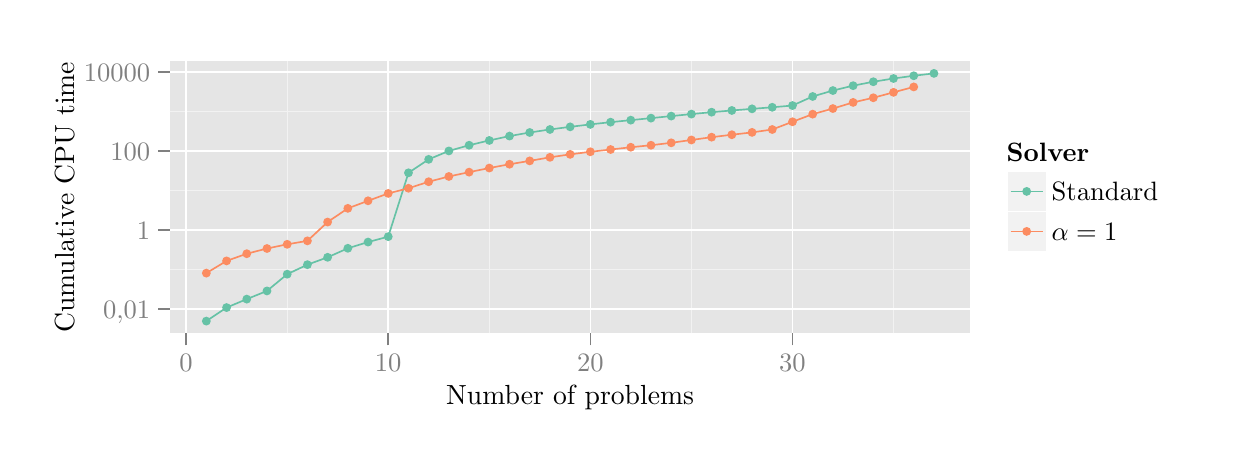
\begin{tikzpicture}[x=1pt,y=1pt]
\definecolor[named]{fillColor}{rgb}{1.00,1.00,1.00}
\path[use as bounding box,fill=fillColor,fill opacity=0.00] (0,0) rectangle (433.62,144.54);
\begin{scope}
\path[clip] (  0.00,  0.00) rectangle (433.62,144.54);
\definecolor[named]{drawColor}{rgb}{1.00,1.00,1.00}
\definecolor[named]{fillColor}{rgb}{1.00,1.00,1.00}

\path[draw=drawColor,line width= 0.6pt,line join=round,line cap=round,fill=fillColor] (  0.00,  0.00) rectangle (433.62,144.54);
\end{scope}
\begin{scope}
\path[clip] ( 51.42, 34.03) rectangle (340.63,132.50);
\definecolor[named]{fillColor}{rgb}{0.90,0.90,0.90}

\path[fill=fillColor] ( 51.42, 34.03) rectangle (340.63,132.50);
\definecolor[named]{drawColor}{rgb}{0.95,0.95,0.95}

\path[draw=drawColor,line width= 0.3pt,line join=round] ( 51.42, 57.08) --
	(340.63, 57.08);

\path[draw=drawColor,line width= 0.3pt,line join=round] ( 51.42, 85.64) --
	(340.63, 85.64);

\path[draw=drawColor,line width= 0.3pt,line join=round] ( 51.42,114.19) --
	(340.63,114.19);

\path[draw=drawColor,line width= 0.3pt,line join=round] ( 93.78, 34.03) --
	( 93.78,132.50);

\path[draw=drawColor,line width= 0.3pt,line join=round] (166.81, 34.03) --
	(166.81,132.50);

\path[draw=drawColor,line width= 0.3pt,line join=round] (239.84, 34.03) --
	(239.84,132.50);

\path[draw=drawColor,line width= 0.3pt,line join=round] (312.87, 34.03) --
	(312.87,132.50);
\definecolor[named]{drawColor}{rgb}{1.00,1.00,1.00}

\path[draw=drawColor,line width= 0.6pt,line join=round] ( 51.42, 42.81) --
	(340.63, 42.81);

\path[draw=drawColor,line width= 0.6pt,line join=round] ( 51.42, 71.36) --
	(340.63, 71.36);

\path[draw=drawColor,line width= 0.6pt,line join=round] ( 51.42, 99.91) --
	(340.63, 99.91);

\path[draw=drawColor,line width= 0.6pt,line join=round] ( 51.42,128.46) --
	(340.63,128.46);

\path[draw=drawColor,line width= 0.6pt,line join=round] ( 57.26, 34.03) --
	( 57.26,132.50);

\path[draw=drawColor,line width= 0.6pt,line join=round] (130.29, 34.03) --
	(130.29,132.50);

\path[draw=drawColor,line width= 0.6pt,line join=round] (203.32, 34.03) --
	(203.32,132.50);

\path[draw=drawColor,line width= 0.6pt,line join=round] (276.36, 34.03) --
	(276.36,132.50);
\definecolor[named]{drawColor}{rgb}{0.40,0.76,0.65}

\path[draw=drawColor,line width= 0.6pt,line join=round] ( 64.56, 38.51) --
	( 71.87, 43.40) --
	( 79.17, 46.45) --
	( 86.47, 49.41) --
	( 93.78, 55.46) --
	(101.08, 58.90) --
	(108.38, 61.56) --
	(115.69, 64.82) --
	(122.99, 67.07) --
	(130.29, 69.03) --
	(137.60, 92.09) --
	(144.90, 96.96) --
	(152.20,100.00) --
	(159.51,102.06) --
	(166.81,103.79) --
	(174.11,105.37) --
	(181.41,106.66) --
	(188.72,107.75) --
	(196.02,108.70) --
	(203.32,109.59) --
	(210.63,110.39) --
	(217.93,111.12) --
	(225.23,111.85) --
	(232.54,112.59) --
	(239.84,113.31) --
	(247.14,114.00) --
	(254.45,114.62) --
	(261.75,115.21) --
	(269.05,115.77) --
	(276.36,116.40) --
	(283.66,119.68) --
	(290.96,121.82) --
	(298.27,123.58) --
	(305.57,125.00) --
	(312.87,126.17) --
	(320.18,127.16) --
	(327.48,128.02);
\definecolor[named]{drawColor}{rgb}{0.99,0.55,0.38}

\path[draw=drawColor,line width= 0.6pt,line join=round] ( 64.56, 55.85) --
	( 71.87, 60.26) --
	( 79.17, 62.86) --
	( 86.47, 64.74) --
	( 93.78, 66.26) --
	(101.08, 67.50) --
	(108.38, 74.30) --
	(115.69, 79.25) --
	(122.99, 81.98) --
	(130.29, 84.65) --
	(137.60, 86.51) --
	(144.90, 88.87) --
	(152.20, 90.77) --
	(159.51, 92.33) --
	(166.81, 93.82) --
	(174.11, 95.19) --
	(181.41, 96.40) --
	(188.72, 97.69) --
	(196.02, 98.76) --
	(203.32, 99.69) --
	(210.63,100.51) --
	(217.93,101.33) --
	(225.23,102.06) --
	(232.54,102.93) --
	(239.84,103.96) --
	(247.14,104.97) --
	(254.45,105.85) --
	(261.75,106.70) --
	(269.05,107.74) --
	(276.36,110.53) --
	(283.66,113.29) --
	(290.96,115.31) --
	(298.27,117.53) --
	(305.57,119.21) --
	(312.87,121.17) --
	(320.18,123.13);
\definecolor[named]{fillColor}{rgb}{0.40,0.76,0.65}

\path[fill=fillColor] ( 64.56, 38.51) circle (  1.60);

\path[fill=fillColor] ( 71.87, 43.40) circle (  1.60);

\path[fill=fillColor] ( 79.17, 46.45) circle (  1.60);

\path[fill=fillColor] ( 86.47, 49.41) circle (  1.60);

\path[fill=fillColor] ( 93.78, 55.46) circle (  1.60);

\path[fill=fillColor] (101.08, 58.90) circle (  1.60);

\path[fill=fillColor] (108.38, 61.56) circle (  1.60);

\path[fill=fillColor] (115.69, 64.82) circle (  1.60);

\path[fill=fillColor] (122.99, 67.07) circle (  1.60);

\path[fill=fillColor] (130.29, 69.03) circle (  1.60);

\path[fill=fillColor] (137.60, 92.09) circle (  1.60);

\path[fill=fillColor] (144.90, 96.96) circle (  1.60);

\path[fill=fillColor] (152.20,100.00) circle (  1.60);

\path[fill=fillColor] (159.51,102.06) circle (  1.60);

\path[fill=fillColor] (166.81,103.79) circle (  1.60);

\path[fill=fillColor] (174.11,105.37) circle (  1.60);

\path[fill=fillColor] (181.41,106.66) circle (  1.60);

\path[fill=fillColor] (188.72,107.75) circle (  1.60);

\path[fill=fillColor] (196.02,108.70) circle (  1.60);

\path[fill=fillColor] (203.32,109.59) circle (  1.60);

\path[fill=fillColor] (210.63,110.39) circle (  1.60);

\path[fill=fillColor] (217.93,111.12) circle (  1.60);

\path[fill=fillColor] (225.23,111.85) circle (  1.60);

\path[fill=fillColor] (232.54,112.59) circle (  1.60);

\path[fill=fillColor] (239.84,113.31) circle (  1.60);

\path[fill=fillColor] (247.14,114.00) circle (  1.60);

\path[fill=fillColor] (254.45,114.62) circle (  1.60);

\path[fill=fillColor] (261.75,115.21) circle (  1.60);

\path[fill=fillColor] (269.05,115.77) circle (  1.60);

\path[fill=fillColor] (276.36,116.40) circle (  1.60);

\path[fill=fillColor] (283.66,119.68) circle (  1.60);

\path[fill=fillColor] (290.96,121.82) circle (  1.60);

\path[fill=fillColor] (298.27,123.58) circle (  1.60);

\path[fill=fillColor] (305.57,125.00) circle (  1.60);

\path[fill=fillColor] (312.87,126.17) circle (  1.60);

\path[fill=fillColor] (320.18,127.16) circle (  1.60);

\path[fill=fillColor] (327.48,128.02) circle (  1.60);
\definecolor[named]{fillColor}{rgb}{0.99,0.55,0.38}

\path[fill=fillColor] ( 64.56, 55.85) circle (  1.60);

\path[fill=fillColor] ( 71.87, 60.26) circle (  1.60);

\path[fill=fillColor] ( 79.17, 62.86) circle (  1.60);

\path[fill=fillColor] ( 86.47, 64.74) circle (  1.60);

\path[fill=fillColor] ( 93.78, 66.26) circle (  1.60);

\path[fill=fillColor] (101.08, 67.50) circle (  1.60);

\path[fill=fillColor] (108.38, 74.30) circle (  1.60);

\path[fill=fillColor] (115.69, 79.25) circle (  1.60);

\path[fill=fillColor] (122.99, 81.98) circle (  1.60);

\path[fill=fillColor] (130.29, 84.65) circle (  1.60);

\path[fill=fillColor] (137.60, 86.51) circle (  1.60);

\path[fill=fillColor] (144.90, 88.87) circle (  1.60);

\path[fill=fillColor] (152.20, 90.77) circle (  1.60);

\path[fill=fillColor] (159.51, 92.33) circle (  1.60);

\path[fill=fillColor] (166.81, 93.82) circle (  1.60);

\path[fill=fillColor] (174.11, 95.19) circle (  1.60);

\path[fill=fillColor] (181.41, 96.40) circle (  1.60);

\path[fill=fillColor] (188.72, 97.69) circle (  1.60);

\path[fill=fillColor] (196.02, 98.76) circle (  1.60);

\path[fill=fillColor] (203.32, 99.69) circle (  1.60);

\path[fill=fillColor] (210.63,100.51) circle (  1.60);

\path[fill=fillColor] (217.93,101.33) circle (  1.60);

\path[fill=fillColor] (225.23,102.06) circle (  1.60);

\path[fill=fillColor] (232.54,102.93) circle (  1.60);

\path[fill=fillColor] (239.84,103.96) circle (  1.60);

\path[fill=fillColor] (247.14,104.97) circle (  1.60);

\path[fill=fillColor] (254.45,105.85) circle (  1.60);

\path[fill=fillColor] (261.75,106.70) circle (  1.60);

\path[fill=fillColor] (269.05,107.74) circle (  1.60);

\path[fill=fillColor] (276.36,110.53) circle (  1.60);

\path[fill=fillColor] (283.66,113.29) circle (  1.60);

\path[fill=fillColor] (290.96,115.31) circle (  1.60);

\path[fill=fillColor] (298.27,117.53) circle (  1.60);

\path[fill=fillColor] (305.57,119.21) circle (  1.60);

\path[fill=fillColor] (312.87,121.17) circle (  1.60);

\path[fill=fillColor] (320.18,123.13) circle (  1.60);
\end{scope}
\begin{scope}
\path[clip] (  0.00,  0.00) rectangle (433.62,144.54);
\definecolor[named]{drawColor}{rgb}{0.50,0.50,0.50}

\node[text=drawColor,anchor=base east,inner sep=0pt, outer sep=0pt, scale=  0.96] at ( 44.30, 39.50) {0,01};

\node[text=drawColor,anchor=base east,inner sep=0pt, outer sep=0pt, scale=  0.96] at ( 44.30, 68.05) {1};

\node[text=drawColor,anchor=base east,inner sep=0pt, outer sep=0pt, scale=  0.96] at ( 44.30, 96.61) {100};

\node[text=drawColor,anchor=base east,inner sep=0pt, outer sep=0pt, scale=  0.96] at ( 44.30,125.16) {10000};
\end{scope}
\begin{scope}
\path[clip] (  0.00,  0.00) rectangle (433.62,144.54);
\definecolor[named]{drawColor}{rgb}{0.50,0.50,0.50}

\path[draw=drawColor,line width= 0.6pt,line join=round] ( 47.15, 42.81) --
	( 51.42, 42.81);

\path[draw=drawColor,line width= 0.6pt,line join=round] ( 47.15, 71.36) --
	( 51.42, 71.36);

\path[draw=drawColor,line width= 0.6pt,line join=round] ( 47.15, 99.91) --
	( 51.42, 99.91);

\path[draw=drawColor,line width= 0.6pt,line join=round] ( 47.15,128.46) --
	( 51.42,128.46);
\end{scope}
\begin{scope}
\path[clip] (  0.00,  0.00) rectangle (433.62,144.54);
\definecolor[named]{drawColor}{rgb}{0.50,0.50,0.50}

\path[draw=drawColor,line width= 0.6pt,line join=round] ( 57.26, 29.77) --
	( 57.26, 34.03);

\path[draw=drawColor,line width= 0.6pt,line join=round] (130.29, 29.77) --
	(130.29, 34.03);

\path[draw=drawColor,line width= 0.6pt,line join=round] (203.32, 29.77) --
	(203.32, 34.03);

\path[draw=drawColor,line width= 0.6pt,line join=round] (276.36, 29.77) --
	(276.36, 34.03);
\end{scope}
\begin{scope}
\path[clip] (  0.00,  0.00) rectangle (433.62,144.54);
\definecolor[named]{drawColor}{rgb}{0.50,0.50,0.50}

\node[text=drawColor,anchor=base,inner sep=0pt, outer sep=0pt, scale=  0.96] at ( 57.26, 20.31) {0};

\node[text=drawColor,anchor=base,inner sep=0pt, outer sep=0pt, scale=  0.96] at (130.29, 20.31) {10};

\node[text=drawColor,anchor=base,inner sep=0pt, outer sep=0pt, scale=  0.96] at (203.32, 20.31) {20};

\node[text=drawColor,anchor=base,inner sep=0pt, outer sep=0pt, scale=  0.96] at (276.36, 20.31) {30};
\end{scope}
\begin{scope}
\path[clip] (  0.00,  0.00) rectangle (433.62,144.54);
\definecolor[named]{drawColor}{rgb}{0.00,0.00,0.00}

\node[text=drawColor,anchor=base,inner sep=0pt, outer sep=0pt, scale=  1] at (196.02,  8.53) {Number of problems};
\end{scope}
\begin{scope}
\path[clip] (  0.00,  0.00) rectangle (433.62,144.54);
\definecolor[named]{drawColor}{rgb}{0.00,0.00,0.00}

\node[text=drawColor,rotate= 90.00,anchor=base,inner sep=0pt, outer sep=0pt, scale=  1] at ( 16.80, 83.26) {Cumulative CPU time};
\end{scope}
\begin{scope}
\path[clip] (  0.00,  0.00) rectangle (433.62,144.54);
\definecolor[named]{fillColor}{rgb}{1.00,1.00,1.00}

\path[fill=fillColor] (349.49, 59.42) rectangle (412.71,107.11);
\end{scope}
\begin{scope}
\path[clip] (  0.00,  0.00) rectangle (433.62,144.54);
\definecolor[named]{drawColor}{rgb}{0.00,0.00,0.00}

\node[text=drawColor,anchor=base west,inner sep=0pt, outer sep=0pt, scale=  0.96] at (353.76, 96.21) {\bfseries Solver};
\end{scope}
\begin{scope}
\path[clip] (  0.00,  0.00) rectangle (433.62,144.54);
\definecolor[named]{drawColor}{rgb}{1.00,1.00,1.00}
\definecolor[named]{fillColor}{rgb}{0.95,0.95,0.95}

\path[draw=drawColor,line width= 0.6pt,line join=round,line cap=round,fill=fillColor] (353.76, 78.15) rectangle (368.22, 92.60);
\end{scope}
\begin{scope}
\path[clip] (  0.00,  0.00) rectangle (433.62,144.54);
\definecolor[named]{drawColor}{rgb}{0.40,0.76,0.65}

\path[draw=drawColor,line width= 0.6pt,line join=round] (355.21, 85.37) -- (366.77, 85.37);
\end{scope}
\begin{scope}
\path[clip] (  0.00,  0.00) rectangle (433.62,144.54);
\definecolor[named]{fillColor}{rgb}{0.40,0.76,0.65}

\path[fill=fillColor] (360.99, 85.37) circle (  1.60);
\end{scope}
\begin{scope}
\path[clip] (  0.00,  0.00) rectangle (433.62,144.54);
\definecolor[named]{drawColor}{rgb}{1.00,1.00,1.00}
\definecolor[named]{fillColor}{rgb}{0.95,0.95,0.95}

\path[draw=drawColor,line width= 0.6pt,line join=round,line cap=round,fill=fillColor] (353.76, 63.69) rectangle (368.22, 78.15);
\end{scope}
\begin{scope}
\path[clip] (  0.00,  0.00) rectangle (433.62,144.54);
\definecolor[named]{drawColor}{rgb}{0.99,0.55,0.38}

\path[draw=drawColor,line width= 0.6pt,line join=round] (355.21, 70.92) -- (366.77, 70.92);
\end{scope}
\begin{scope}
\path[clip] (  0.00,  0.00) rectangle (433.62,144.54);
\definecolor[named]{fillColor}{rgb}{0.99,0.55,0.38}

\path[fill=fillColor] (360.99, 70.92) circle (  1.60);
\end{scope}
\begin{scope}
\path[clip] (  0.00,  0.00) rectangle (433.62,144.54);
\definecolor[named]{drawColor}{rgb}{0.00,0.00,0.00}

\node[text=drawColor,anchor=base west,inner sep=0pt, outer sep=0pt, scale=  0.96] at (370.02, 82.07) {Standard};
\end{scope}
\begin{scope}
\path[clip] (  0.00,  0.00) rectangle (433.62,144.54);
\definecolor[named]{drawColor}{rgb}{0.00,0.00,0.00}

\node[text=drawColor,anchor=base west,inner sep=0pt, outer sep=0pt, scale=  0.96] at (370.02, 67.61) {\(\alpha=1\)};
\end{scope}
\end{tikzpicture}

	\end{figcenter}
	\caption{Accumulated runtime of the standard and greedy algorithm in the \emph{Black Hole} set, sorted by runtime individually for each variant. Note the logarithmic scale of the \(y\) axis.}
	\label{fig:cactus-greedy}
\end{figure}

\Cref{fig:cactus-greedy} illustrates the utility of the greedy DP update.
While it is slower for very small problems in the \emph{Black Hole} set, it is significantly faster in solving the more difficult problems.

The only set in which the greedy update performs significantly worse is the \emph{Auction} set, in which it fails to solve any problems at all.

% Note: for some problems, including CFN/ProteinDesign, no loss in accuracy but great decrease in time - discuss this!

% [todo] - more observations?
